% Options for packages loaded elsewhere
\PassOptionsToPackage{unicode}{hyperref}
\PassOptionsToPackage{hyphens}{url}
%
\documentclass[
  10pt,
  a4paper]{article}
\title{Analysis 1B --- Tutorial 3}
\author{Christian Jones: University of Bath}
\date{February 2023}

\usepackage{amsmath,amssymb}
\usepackage{lmodern}
\usepackage{iftex}
\ifPDFTeX
  \usepackage[T1]{fontenc}
  \usepackage[utf8]{inputenc}
  \usepackage{textcomp} % provide euro and other symbols
\else % if luatex or xetex
  \usepackage{unicode-math}
  \defaultfontfeatures{Scale=MatchLowercase}
  \defaultfontfeatures[\rmfamily]{Ligatures=TeX,Scale=1}
\fi
% Use upquote if available, for straight quotes in verbatim environments
\IfFileExists{upquote.sty}{\usepackage{upquote}}{}
\IfFileExists{microtype.sty}{% use microtype if available
  \usepackage[]{microtype}
  \UseMicrotypeSet[protrusion]{basicmath} % disable protrusion for tt fonts
}{}
\makeatletter
\@ifundefined{KOMAClassName}{% if non-KOMA class
  \IfFileExists{parskip.sty}{%
    \usepackage{parskip}
  }{% else
    \setlength{\parindent}{0pt}
    \setlength{\parskip}{6pt plus 2pt minus 1pt}}
}{% if KOMA class
  \KOMAoptions{parskip=half}}
\makeatother
\usepackage{xcolor}
\IfFileExists{xurl.sty}{\usepackage{xurl}}{} % add URL line breaks if available
\IfFileExists{bookmark.sty}{\usepackage{bookmark}}{\usepackage{hyperref}}
\hypersetup{
  pdftitle={Analysis 1B --- Tutorial 3},
  pdfauthor={Christian Jones: University of Bath},
  hidelinks,
  pdfcreator={LaTeX via pandoc}}
\urlstyle{same} % disable monospaced font for URLs
\usepackage[margin=2.5cm]{geometry}
\usepackage{longtable,booktabs,array}
\usepackage{calc} % for calculating minipage widths
% Correct order of tables after \paragraph or \subparagraph
\usepackage{etoolbox}
\makeatletter
\patchcmd\longtable{\par}{\if@noskipsec\mbox{}\fi\par}{}{}
\makeatother
% Allow footnotes in longtable head/foot
\IfFileExists{footnotehyper.sty}{\usepackage{footnotehyper}}{\usepackage{footnote}}
\makesavenoteenv{longtable}
\usepackage{graphicx}
\makeatletter
\def\maxwidth{\ifdim\Gin@nat@width>\linewidth\linewidth\else\Gin@nat@width\fi}
\def\maxheight{\ifdim\Gin@nat@height>\textheight\textheight\else\Gin@nat@height\fi}
\makeatother
% Scale images if necessary, so that they will not overflow the page
% margins by default, and it is still possible to overwrite the defaults
% using explicit options in \includegraphics[width, height, ...]{}
\setkeys{Gin}{width=\maxwidth,height=\maxheight,keepaspectratio}
% Set default figure placement to htbp
\makeatletter
\def\fps@figure{htbp}
\makeatother
\setlength{\emergencystretch}{3em} % prevent overfull lines
\providecommand{\tightlist}{%
  \setlength{\itemsep}{0pt}\setlength{\parskip}{0pt}}
\setcounter{secnumdepth}{5}
\newcommand{\BOO}{BOO}
\usepackage {hyperref}
\hypersetup {colorlinks = true, linkcolor = blue, urlcolor = blue}
\usepackage{float}
\ifLuaTeX
  \usepackage{selnolig}  % disable illegal ligatures
\fi

\usepackage{amsthm}
\theoremstyle{plain}
\newtheorem*{theorem*}{Theorem}\newtheorem{theorem}{Theorem}[section]
\theoremstyle{definition}
\newtheorem*{definition*}{Definition}\newtheorem{definition}{Definition}[section]
\theoremstyle{plain}
\newtheorem*{proposition*}{Proposition}\newtheorem{proposition}[theorem]{Proposition}
\newtheorem*{Definitions*}{Definitions}\newtheorem{Definitions}[definition]{Definitions}
\theoremstyle{plain}
\newtheorem*{lemma*}{Lemma}\newtheorem{lemma}{Lemma}[section]
\theoremstyle{plain}
\newtheorem*{corollary*}{Corollary}\newtheorem{corollary}{Corollary}[section]
\theoremstyle{plain}
\newtheorem*{conjecture*}{Conjecture}\newtheorem{conjecture}{Conjecture}[section]
\theoremstyle{definition}
\newtheorem*{example*}{Example}\newtheorem{example}{Example}[section]
\theoremstyle{definition}
\newtheorem*{exercise*}{Exercise}\newtheorem{exercise}{Exercise}[section]
\newtheorem*{Thought*}{Thought}\newtheorem{Thought}{Thought}[section]
\theoremstyle{remark}
\newtheorem*{remark*}{Remark}
\newtheorem*{solution*}{Solution}
\newtheorem*{Example*}{Example}
\theoremstyle{remark}
\newtheorem*{Proof*}{Proof}
\newtheorem*{Examples*}{Examples}
\let\BeginKnitrBlock\begin \let\EndKnitrBlock\end
\begin{document}
\maketitle

{
\setcounter{tocdepth}{2}
\tableofcontents
}
\newpage
\pagenumbering{arabic}

\hypertarget{introduction}{%
\section*{Introduction}\label{introduction}}
\addcontentsline{toc}{section}{Introduction}

Here is the material to accompany the 3rd Analysis 1B Tutorial on the 20th February. Alternative formats can be downloaded by clicking the download icon at the top of the page. Please send any comments or corrections to \href{mailto:caj50@bath.ac.uk}{Christian Jones (caj50)}. To return to the homepage, click \href{http://caj50.github.io/tutoring.html}{here}.

\hypertarget{lecture-recap}{%
\section{Lecture Recap}\label{lecture-recap}}

\hypertarget{algebra-of-limits-for-functions}{%
\subsection{Algebra of Limits for Functions}\label{algebra-of-limits-for-functions}}

From last week, recall that we showed that we can characterise the limit of a function at a point in terms of sequences. This was brilliant, as it allowed us to apply the theory we derived in Semester 1 directly to functions. In particular, this gives us an easy way of finding the limits of sums and products of functions:

\BeginKnitrBlock{theorem}[Algebra of Limits]
{\label{thm:thm1} }Let \(c, L, M, \lambda \in \mathbb{R}\), and let \(f,g: D \to \mathbb{R}\), where \(D\) is a punctured neighbourhood of \(c\). Suppose \(\lim_{x \to c}f(x) = L\), and \(\lim_{x \to c}g(x) = M\). Then:

\begin{enumerate}
\def\labelenumi{\arabic{enumi}.}
\item
  \(\lim_{x\to c}\left(f \pm g\right)(x) = L \pm M,\)
\item
  \(\lim_{x \to c}\lambda f(x) = \lambda L,\)
\item
  \(\lim_{x \to c}(fg)(x) = LM,\)
\item
  If \(g(x) \neq 0 \;\;\forall x \in D\), and \(M \neq 0\), then \[\lim_{x \to c}\left(\frac{f}{g}\right)(x) = \frac{L}{M}.\]
\end{enumerate}
\EndKnitrBlock{theorem}

Note that here, we define the \emph{product} of \(f\) and \(g\) by \((fg)(x) = f(x)g(x)\) --- don't get this confused with the composition \((f \circ g)(x) = f(g(x))\)!

\hypertarget{left-and-right-limits}{%
\subsection{Left and Right Limits}\label{left-and-right-limits}}

When finding the limit of a function \(f\) at a point \(c\) in the interior of its domain, we are free to approach \(c\) from whichever direction we like. However, we could equally restrict ourselves to approaching \(c\) only from the left or the right, and observing how the function values respond. This gives rise to the idea of \emph{left and right hand limits}.

\BeginKnitrBlock{definition}[Left and Right Hand Limits]
{\label{def:def1} }Let \(c, L, M \in \mathbb{R}\), and let \(f: D \to \mathbb{R}\).

\begin{enumerate}
\def\labelenumi{\arabic{enumi}.}
\tightlist
\item
  Suppose \(\exists \delta_0 > 0\) such that \((c, c + \delta_0) \subseteq D\). Then \(\lim_{x \to c^{+}}f(x) = L\) means that \[\forall \epsilon >0\;\;\exists \delta>0\;\;\text{s.t}\;\; \forall x \in D,\;\; 0 < x - c < \delta \Rightarrow \lvert f(x) - L \rvert < \epsilon.\] This is the \emph{right-hand limit} at \(c\).
\item
  Suppose \(\exists \delta_0 > 0\) such that \((c - \delta_0, c) \subseteq D\). Then \(\lim_{x \to c^{-}}f(x) = M\) means that \[\forall \epsilon >0\;\;\exists \delta>0\;\;\text{s.t}\;\; \forall x \in D,\;\; 0 < x - c < \delta \Rightarrow \lvert f(x) - M \rvert < \epsilon.\] This is the \emph{left-hand limit} at \(c\).
\end{enumerate}
\EndKnitrBlock{definition}

As the names suggest, we approach \(c\) from the left when calculating the left-hand limit, and we approach \(c\) from the right when calculating the right-hand limit. It also turns out that these objects can be very useful in calculating function limits, especially when the function is defined piecewise:

\BeginKnitrBlock{proposition}
{\label{prp:prop1} }Let \(c \in \mathbb{R}\), and let \(f: D \to \mathbb{R}\), where \(D\) is a punctured neighbourhood of \(c\). Then \(\lim_{x \to c}f(x)\) exists if and only if both the left and right hand limits exist, and are equal.
\EndKnitrBlock{proposition}

Finally, note that if we had a function on a domain such as \(D = [-1,2]\), we could only search for the right hand limit at \(c = -1\), and the left hand limit at \(c = 2\). This is because there is no way we could approach these elements of the domain from the left or right respectively.

\hypertarget{continuity}{%
\subsection{Continuity}\label{continuity}}

A stronger statement than requiring a function to have a limit at a value \(c\) is for that function to be continuous. Up until now, you may have thought of a continuous function as one that can be drawn without taking your pen off the page. We can make that idea more precise in the following definition:

\BeginKnitrBlock{definition}[Continuity]
{\label{def:def2} }Let \(D \subseteq \mathbb{R}\), and \(f: D \to \mathbb{R}\). Then \(f\) is continuous at a point \(c\) if \[\forall \epsilon > 0\;\;\exists \delta > 0\;\;\text{s.t.}\;\;\forall x \in D,\;\; \lvert x - c \rvert < \delta \Rightarrow \lvert f(x) - f(c) \rvert < \epsilon.\]
\EndKnitrBlock{definition}

A graphical example of this definition can be seen in Figure \ref{fig:cont}.

\begin{figure}
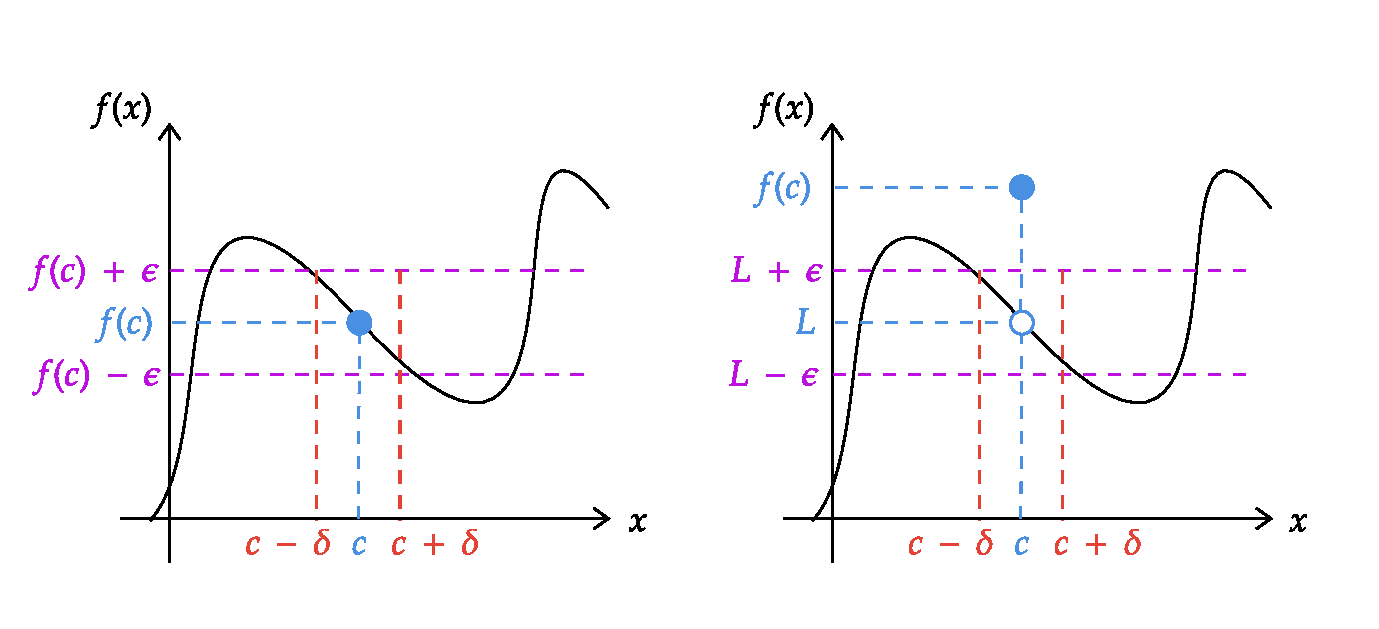
\includegraphics{Continuity} \caption{A diagram illustrating the definition of a continuous function at a point $c$ (left). Compare this to a function which only approaches a limit $L$ as $x \to c$ (right).}\label{fig:cont}
\end{figure}

You might be thinking that this looks remarkably like the definition of a limit from last week, and you would be right. In fact: \[f\;\;\text{is continuous at}\;\; c \Longleftrightarrow \lim_{x \to c}f(x) = f(c).\] However, note that we require \(f\) to be defined at \(c\) for \(f\) to be continuous; in the limit definition, we didn't care whether or not \(f(c)\) existed.

\hypertarget{hints}{%
\section{Hints}\label{hints}}

As per usual, here's where you'll find the problem sheet hints!

\begin{enumerate}
\def\labelenumi{\arabic{enumi})}
\tightlist
\item
  Part a) is all about using the epsilon-delta definition of limit. Firstly, note that there are two things to prove here because of the `if and only if'. Think about how you can substitute variables to move from the definition of one limit to the definition of the other. For part b), think about using a step function for \(f\).
\item
  Again, this is all about manipulating an unfamiliar definition, and again, there are two things to prove! Pretty much the same idea applies here too --- try and rewrite one definition so it starts to look like the other, then use that to make a choice of \(\delta\) and/or \(M\) (depending on which implication you are proving).
\item
  This is quite similar to the example we did in tutorials. Note that you'll have to take cases on \(x\) when evaluating \(\lvert f(x) - f(0)\rvert\), but in both cases, you'll end up with the same bound in terms of \(\delta\).
\end{enumerate}

\end{document}
